\chapter{General introduction}
%\addcontentsline{toc}{chapter}{Introduction}
\markboth{}{General introduction}
\epigraph{\emph{History, as well as life itself, is complicated; neither life nor history is an enterprise for those who seek simplicity and consistency}}{\cite{Diamond2005}}
\label{C01}

\section{Introduction}
\label{C01_01}

The loss of biodiversity is of increasing concern worldwide because of its value to humankind. Biodiversity, the variability of organisms and the ecological complexes they are part of \citep{SecretariatoftheConventiononBiologicalDiversity2014}, is constantly changing, with the number of extant species in many taxonomic groups \textendash\ such as birds \citep{Jetz2012} or mammals \citep{Upham2019} \textendash\ varying in space and time. However current global extinction rates have been estimated to be 100 to 1000 times higher than natural background rates \citep{Pimm2014}, resulting in the Earth loosing most of its megafauna and many other species \citep{Sandom2014,Ceballos2017,Hallmann2017}, including those endemic to islands \citep{Blackburn2004} or with certain ecological traits \citep{Fritz2009}. Increasingly humankind realizes that further losses of biodiversity would be detrimental, either because of its intrinsic value or because of the realization that ecosystem functions and services are essential for human and economic wellbeing \citep{Cardinale2012,Mace2014}. For instance it has been shown that the loss of biodiversity \textendash\ particularly at local scales \textendash\ may be correlated with a loss of ecosystem functions and services \citep{Albrecht2014,Oliver2015,Hautier2015,Isbell2015}. There are multiple pressures on biodiversity globally \citep{Butchart2010,Steffen2015}, but establishing links between biodiversity loss and thoe pressures is often challenging \citep{Cardinale2018,DePalma2018}.

% Cool info box
%\begin{wrapfigure}{r}{1\textwidth}
  \vspace{-20pt}
  \begin{center}
        \begin{definitions}[Definitions]
        This thesis follows the definitions by \cite{Lambin2006}, who define \textbf{land cover} as the \textbf{conditions} of the Earth’s \textbf{land surface} including abiotic and biotic structures. In contrast \textbf{land use} has been defined as the purposes to which humans exploit and manipulate land cover \citep{Lambin2006}. Satellite-based remote sensing is capable (see \ref{C01_0101}) of monitoring land-surface conditions, \ie land cover, but is usually unable to identify land use \textit{per se}. Land use and land cover often form a coupled human-environmental \textbf{land system} \citep{Lambin2006,Turner2007} and as a unifying framework the term \textbf{land change} recognizes that changes in land-use and/or land-cover can often not be separated \citep{Turner2007,Lambin2006}.
        \end{definitions}  
  \end{center}
  \vspace{-20pt}
%\end{wrapfigure}

Land change \textendash\ defined as change in land use and/or land cover caused by natural or anthropogenic factors \citep[Box 1.1, ][]{Lambin2003,Turner2007,Song2018} \textendash\ is among the main drivers of biodiversity loss across scales. Among 8,688 species listed in the International Union for Conservation of Nature (IUCN) Red List, 62.2\% of species globally are threatened with extinction because of agricultural activities and 34.7\% by urban development \citep{Maxwell2016}. Across biomes, vertebrate richness \citep{Brum2013,Kehoe2017} and distribution \citep{DiMarco2015} can best be explained by the occurrence of anthropogenically altered land. Broad-scale syntheses found differences in land use and/or land cover to impact local biodiversity globally \citep{Gibson2011,Murphy2014,Newbold2014b,Newbold2015,Alroy2017} with local species richness estimated to be reduced by 13\% globally relative to undisturbed primary vegetation \citep{Newbold2015}, increasingly exceeding planetary boundaries \citep{Newbold2016a}. Impacts of land change are furthermore dependent on functional traits of species \citep{Newbold2013,Jung2016} with species of large body size \citep{Newbold2013,Newbold2015} or narrow range \citep{Newbold2018} being particularly affected. However, these broad-scale syntheses primarily investigated the impacts of spatial differences in land-use/land-cover at the time of biodiversity sampling \citep{Gibson2011,Murphy2014,Newbold2015,Alroy2017}. Land changes that occurred before biodiversity sampling are often ignored, despite published evidence of their impacts on local biodiversity.

Past land changes continue to influence local biodiversity \citep{Foster2003}. These influences are detectable in altered soil biodiversity \citep{Jakovac2016,Wood2017}, vegetation growth \citep{Fraterrigo2006} or species composition \citep{Bellemare2002,Ewers2013,Jakovac2016}. After a land change, biodiversity can recover \citep{Chazdon2003} depending on key attributes of land change (see \ref{C01_0103} for further detail) such as magnitude or time passed \citep{Martin2013,Fu2017,Jones2018}. However previous evidence on lasting impacts of past land change is not consistent, reporting either losses \citep{Moreno-Mateos2017,Jones2018}, mixed changes \citep{Svensson2012,Thom2016} or increases \citep{Fu2017} in local biodiversity measures [predominantly species richness]. Furthermore, these studies investigated only a single attribute of land change, \eg time passed, while those that assessed multiple attributes \citep{Shackelford2017} surprisingly found most attributes to be not important in explaining differences in biodiversity.

Overall there remain several gaps in our knowledge of how land change affects local biodiversity: Importantly (\textit{i}) most previous broad-scale syntheses only coarsely - if at all - considered land changes in the past \citep{Alkemade2009,Murphy2014,Newbold2015} and corresponding lasting effects (see \ref{C01_0103}) on local biodiversity \citep{Dullinger2013,Hylander2013}; (\textit{ii}) past land change has often been inferred from anecdotal, non-replicable information \textendash\ \ie encoded as “secondary vegetation” \citep{Hudson2014} or “abandoned agriculture” \citep{Gibson2011} \textendash\ or land use/land-cover data from extrapolated estimates \citep{Hurtt2011}, impeding external validation and quantification of land change attributes; and (\textit{iii}) many previous studies investigating impacts of past land change on biodiversity focussed on specific geographic regions \citep{Bellemare2002,Ewers2013,Cousins2015}, taxonomic groups \citep{Hermy2007,Perring2018} or single biodiversity measure such as species richness \citep{Martin2013,Fu2017}, which has been shown to be problematic \citep{Su2004,Hillebrand2017}, rather than providing a comparative and comprehensive assessment globally. Here I will address these gaps by investigating if and how local biodiversity differs because of past land changes \textendash\ quantified by satellite-based remote sensing (Figure \ref{F01_01}) \textendash\ and what attributes might drive these differences in biodiversity measures.


\subsection{Land change in the Anthropocene}
\label{C01_0101}

Land is always changing. Change can happen because of a variety of factors that vary across spatial and temporal scales \citep{Lambin2003,Kennedy2014}. Some natural events such as flooding, storms or plant diseases alter land cover infrequently \citep{Turner1998}, while others \textendash\ such as repeated droughts or frequent wildfires \textendash\ can define and shape entire ecoregions. Such is the case for the North American Midwest or South African Fynbos ecoregions which are characterized by frequent wildfires \citep{Westerling2006,Kelly2017}. In rare instances natural factors can change entire biomes. The Sahara desert, covered by forests and savanna grasslands until 18,000 years B.P., has lost most of its natural vegetation because of changes in precipitation cycles \citep{Hamilton1981}. Yet, those extensive natural land changes are dwarfed by the pervasive impacts humans have on the Earth’s surface and there is an increasing realization that any characterization of terrestrial biomes is incomplete without acknowledging the influence of humans \citep{Ellis2008,Kehoe2017}.

Humankind continues to shape the land \citep{Ellis2011,Ellis2013} with human-driven land changes occurring since 10,000 years B.P \citep{Ellis2013}. Evidence of agricultural activities from ancient civilizations are noticeable even in the most remote places such as the Amazon basin \citep{McMichael2017}. Europe, once predominantly covered by forests, has lost most natural vegetation in the Middle Ages and early Renaissance \citep{Kaplan2009}, resulting in the human-dominated landscapes of the present. Land changes in those landscapes occur frequently \citep{Kleyer2007}, with the dominant land cover alternating between grass-, crop- and shrub-covered land \citep{Kleyer2007,Manning2009}. The temporal acceleration of anthropogenic factors altering the Earth surface \citep{Steffen2015} have led researchers to declare a new geological epoch, the “Anthropocene”, varyingly dated to have started as early as 3000 years B.P. or as late as the 20\textsuperscript{th} century \citep{Ellis2013a}. 

Most of the knowledge of pre-20\textsuperscript{th} century land change is derived from soil cores, historic texts, archaeological evidence or photographs and drawings \citep{KleinGoldewijk2011,KleinGoldewijk2016}. While these sources remain the best and often only data available, reconstructions of past land change rely on multiple assumptions \citep{KleinGoldewijk2013} and, when projected in space and time, can often be very different from independent soil-core based land cover reconstructions \citep{Kaplan2017}. For more recent time periods and as an alternative to reconstructed land change, satellite-based remote sensing directly measures the conditions of the Earth's land surface (Box 1).

% ---------------- Figure 1 --------------------- %
\begin{figure}[htb]
\centering
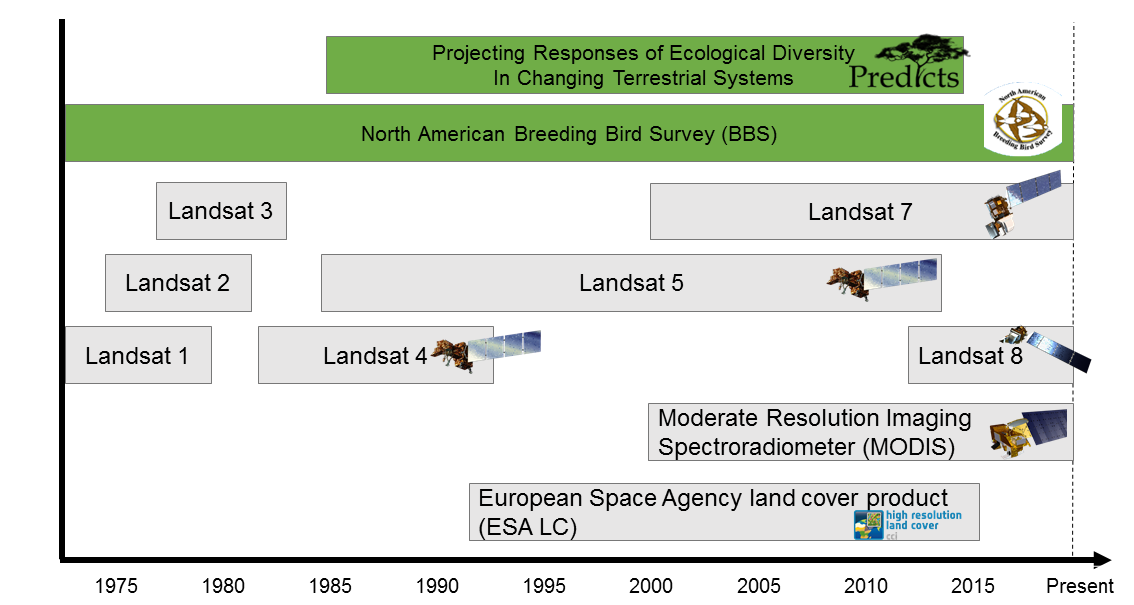
\includegraphics[width=1\textwidth]{chapter1/F01}
\caption{ Temporal coverage of biodiversity (green) and remote sensing (grey) datasets used in this thesis. Legacy Landsat missions (1-3) are shown for completeness only. }
\label{F01_01}
\end{figure}
% -------------------------------------------- %

Through technological advances humans have created a global spaceborne Earth observation system. The first satellite missions were used exclusively for military intelligence or weather observations. Since the mid-1970s satellite missions (Figure \ref{F01_01}), such as Landsat or later the Terra \& Aqua satellites with the Moderate Resolution Imaging Spectroradiometer (MODIS) sensor, were specifically designed to repeatedly photograph the Earth on a global scale \citep{Schaaf2002,Zhang2006,Kennedy2014}. These satellites carry highly sensitive sensors that measure the spectral reflectance from solar insolation. The near-infrared spectrum (Figure \ref{F01_02}\textbf{a}) has been recognized to be particularly useful for monitoring the photosynthetic activity of vegetation and can be quantified through “vegetation indices” \citep{Tucker1979,Tucker1981,Pettorelli2005,Jiang2008}. Differences in the dynamics of vegetation indices (Figure \ref{F01_02}\textbf{b}-\textbf{c}) can be used to identify land change globally. 

% ---------------- Figure 2 --------------------- %
\begin{figure}[htb]
\centering
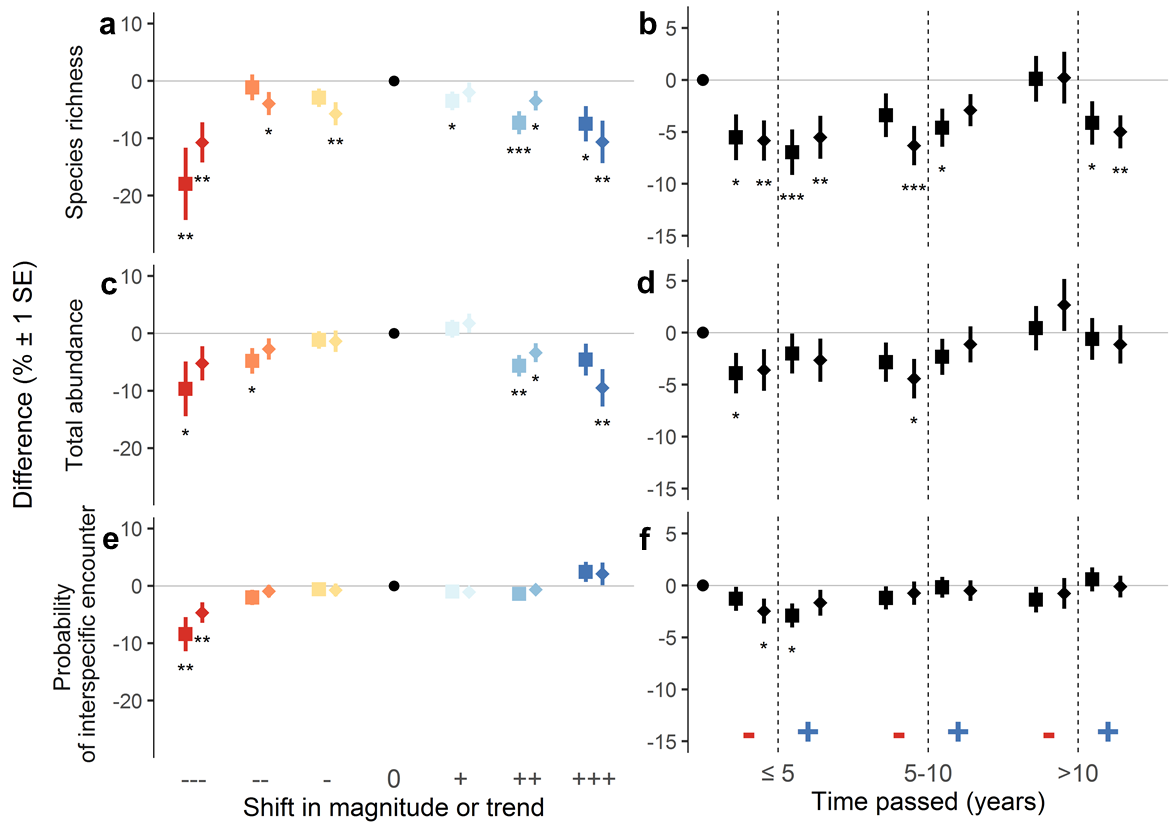
\includegraphics[width=1\textwidth]{chapter1/F02}
\caption{ (\textbf{a}) Schematic of how differences in spectral reflectances assist distinguishing leaf colour. (\textbf{b}) Map (Centre longitude: $0.165$\textdegree, latitude: $50.778$\textdegree) shows an annual maximum value composite (MVC) for 2018 of the Enhanced Vegetation Index (EVI) as calculated from the Landsat 8 mission. (\textbf{c}) Monthly MVC time series of three example sites (black points highlighted in \textbf{c}) of known land cover (cultivated land, forest, semi-natural grassland). }
\label{F01_02}
\end{figure}
% -------------------------------------------- %

Land change can be monitored using satellite-based remote sensing. A change on land can occur as either ‘conversion’ or ‘modification’, where the former is usually understood as “complete replacement of one land-cover type by another” \textendash\ \ie deforestation \textendash\ while the latter are “subtle changes” \textendash\ \ie agricultural intensification \textendash\ that affect the character of a land cover \citep{Lambin2003,Lambin2006}. Spatial estimates of the Earth’s land cover are commonly derived through a classification of remotely-sensed spectral reflectances \citep{DeFries1994,Hansen2000,DiGregorio2000}. However, these spatial estimates could often not be temporally compared because of classification biases and thematic inconsistencies \citep{VERBURG2011,Estes2018} and \textendash\ until recently \textendash\ little progress has been made to quantify land change globally. Novel algorithms and processing frameworks have been developed to quantify land change from temporal dynamics of spectral reflectances measuring photosynthetic activity \citep[Figure \ref{F01_02}\textbf{c}, ][]{Lhermitte2011,Gomez2016,Zhu2017}. With increasing availability and accessibility of satellite data \citep{Wulder2015} and computational power \citep{Gorelick2017} land changes have been quantified globally \citep{Hansen2013,Pekel2016,Li2018,Song2018}, creating new opportunities to  assess impacts of land change on biodiversity.   


\subsection{The impacts of past land change on local biodiversity}
\label{C01_0102}

% ---------------- Figure 3 --------------------- %
\begin{wrapfigure}{r}{0.5\textwidth}
  \begin{flushright}
    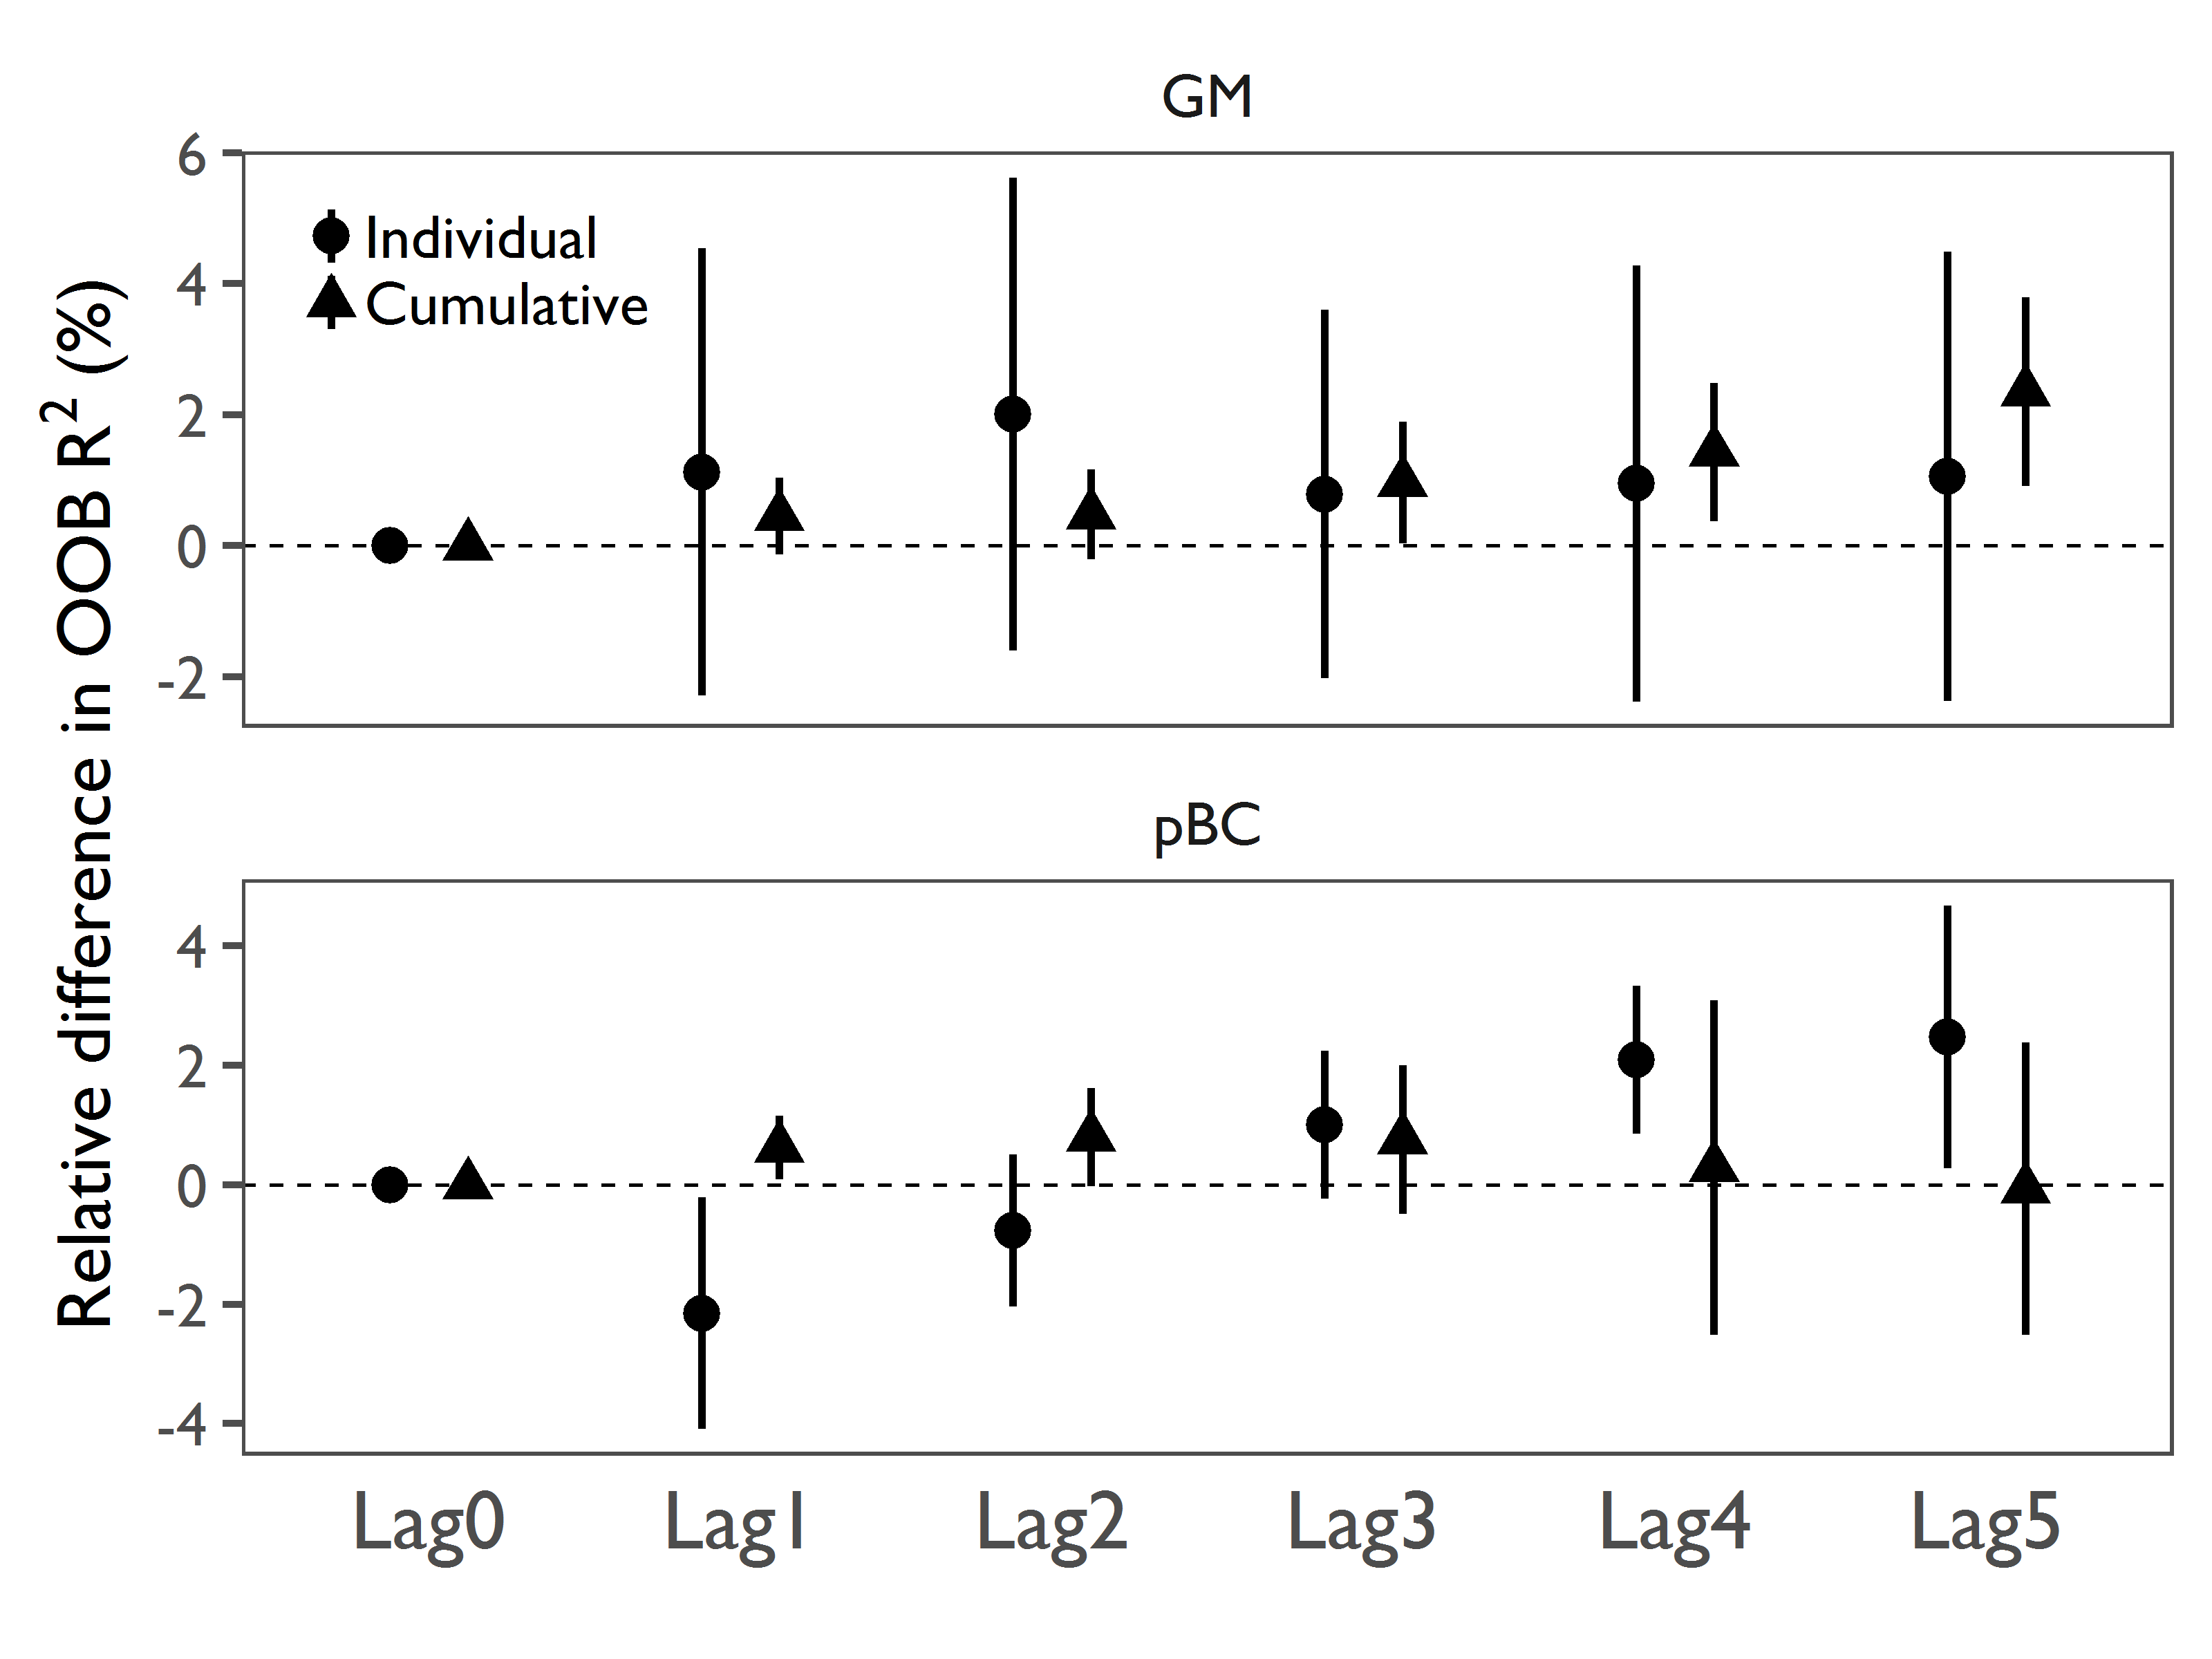
\includegraphics[width=.5\textwidth]{chapter1/F03}
  \end{flushright}
  \caption{ Schematic how a biodiversity response variable (red) can be estimated using environmental predictors (blue) in space and time. Adapted from \cite{Ferrier2017}. }
  \label{F01_03}
\end{wrapfigure}
% -------------------------------------------- %

Land changes can have immediate and/or delayed impacts on local biodiversity. They can act as disturbance affecting the stability of an ecosystem \citep{Pimm1984,Scheffer2003}, causing an immediate reduction in the number of species and individuals \citep{Nimmo2015,Ratajczak2018}. In addition, land changes can have delayed impacts on local biodiversity that persist for decades \citep{Martin2013,Moreno-Mateos2017} or centuries \citep{Vegas-Vilarrubia2011,McMichael2017}. Previous studies that investigated lasting influences of past land change \textendash\ varyingly described as “land-use history” or “landscape history” \citep{Bellemare2002,Foster2003,Ewers2013} or “management legacies” \citep{Perring2015} \textendash\ on biodiversity explained these influences through a number of mechanisms (Figure \ref{F01_04}, Table \ref{T01_01}).

% ---------------- Figure 4 --------------------- %
\begin{figure}[htb]
\centering
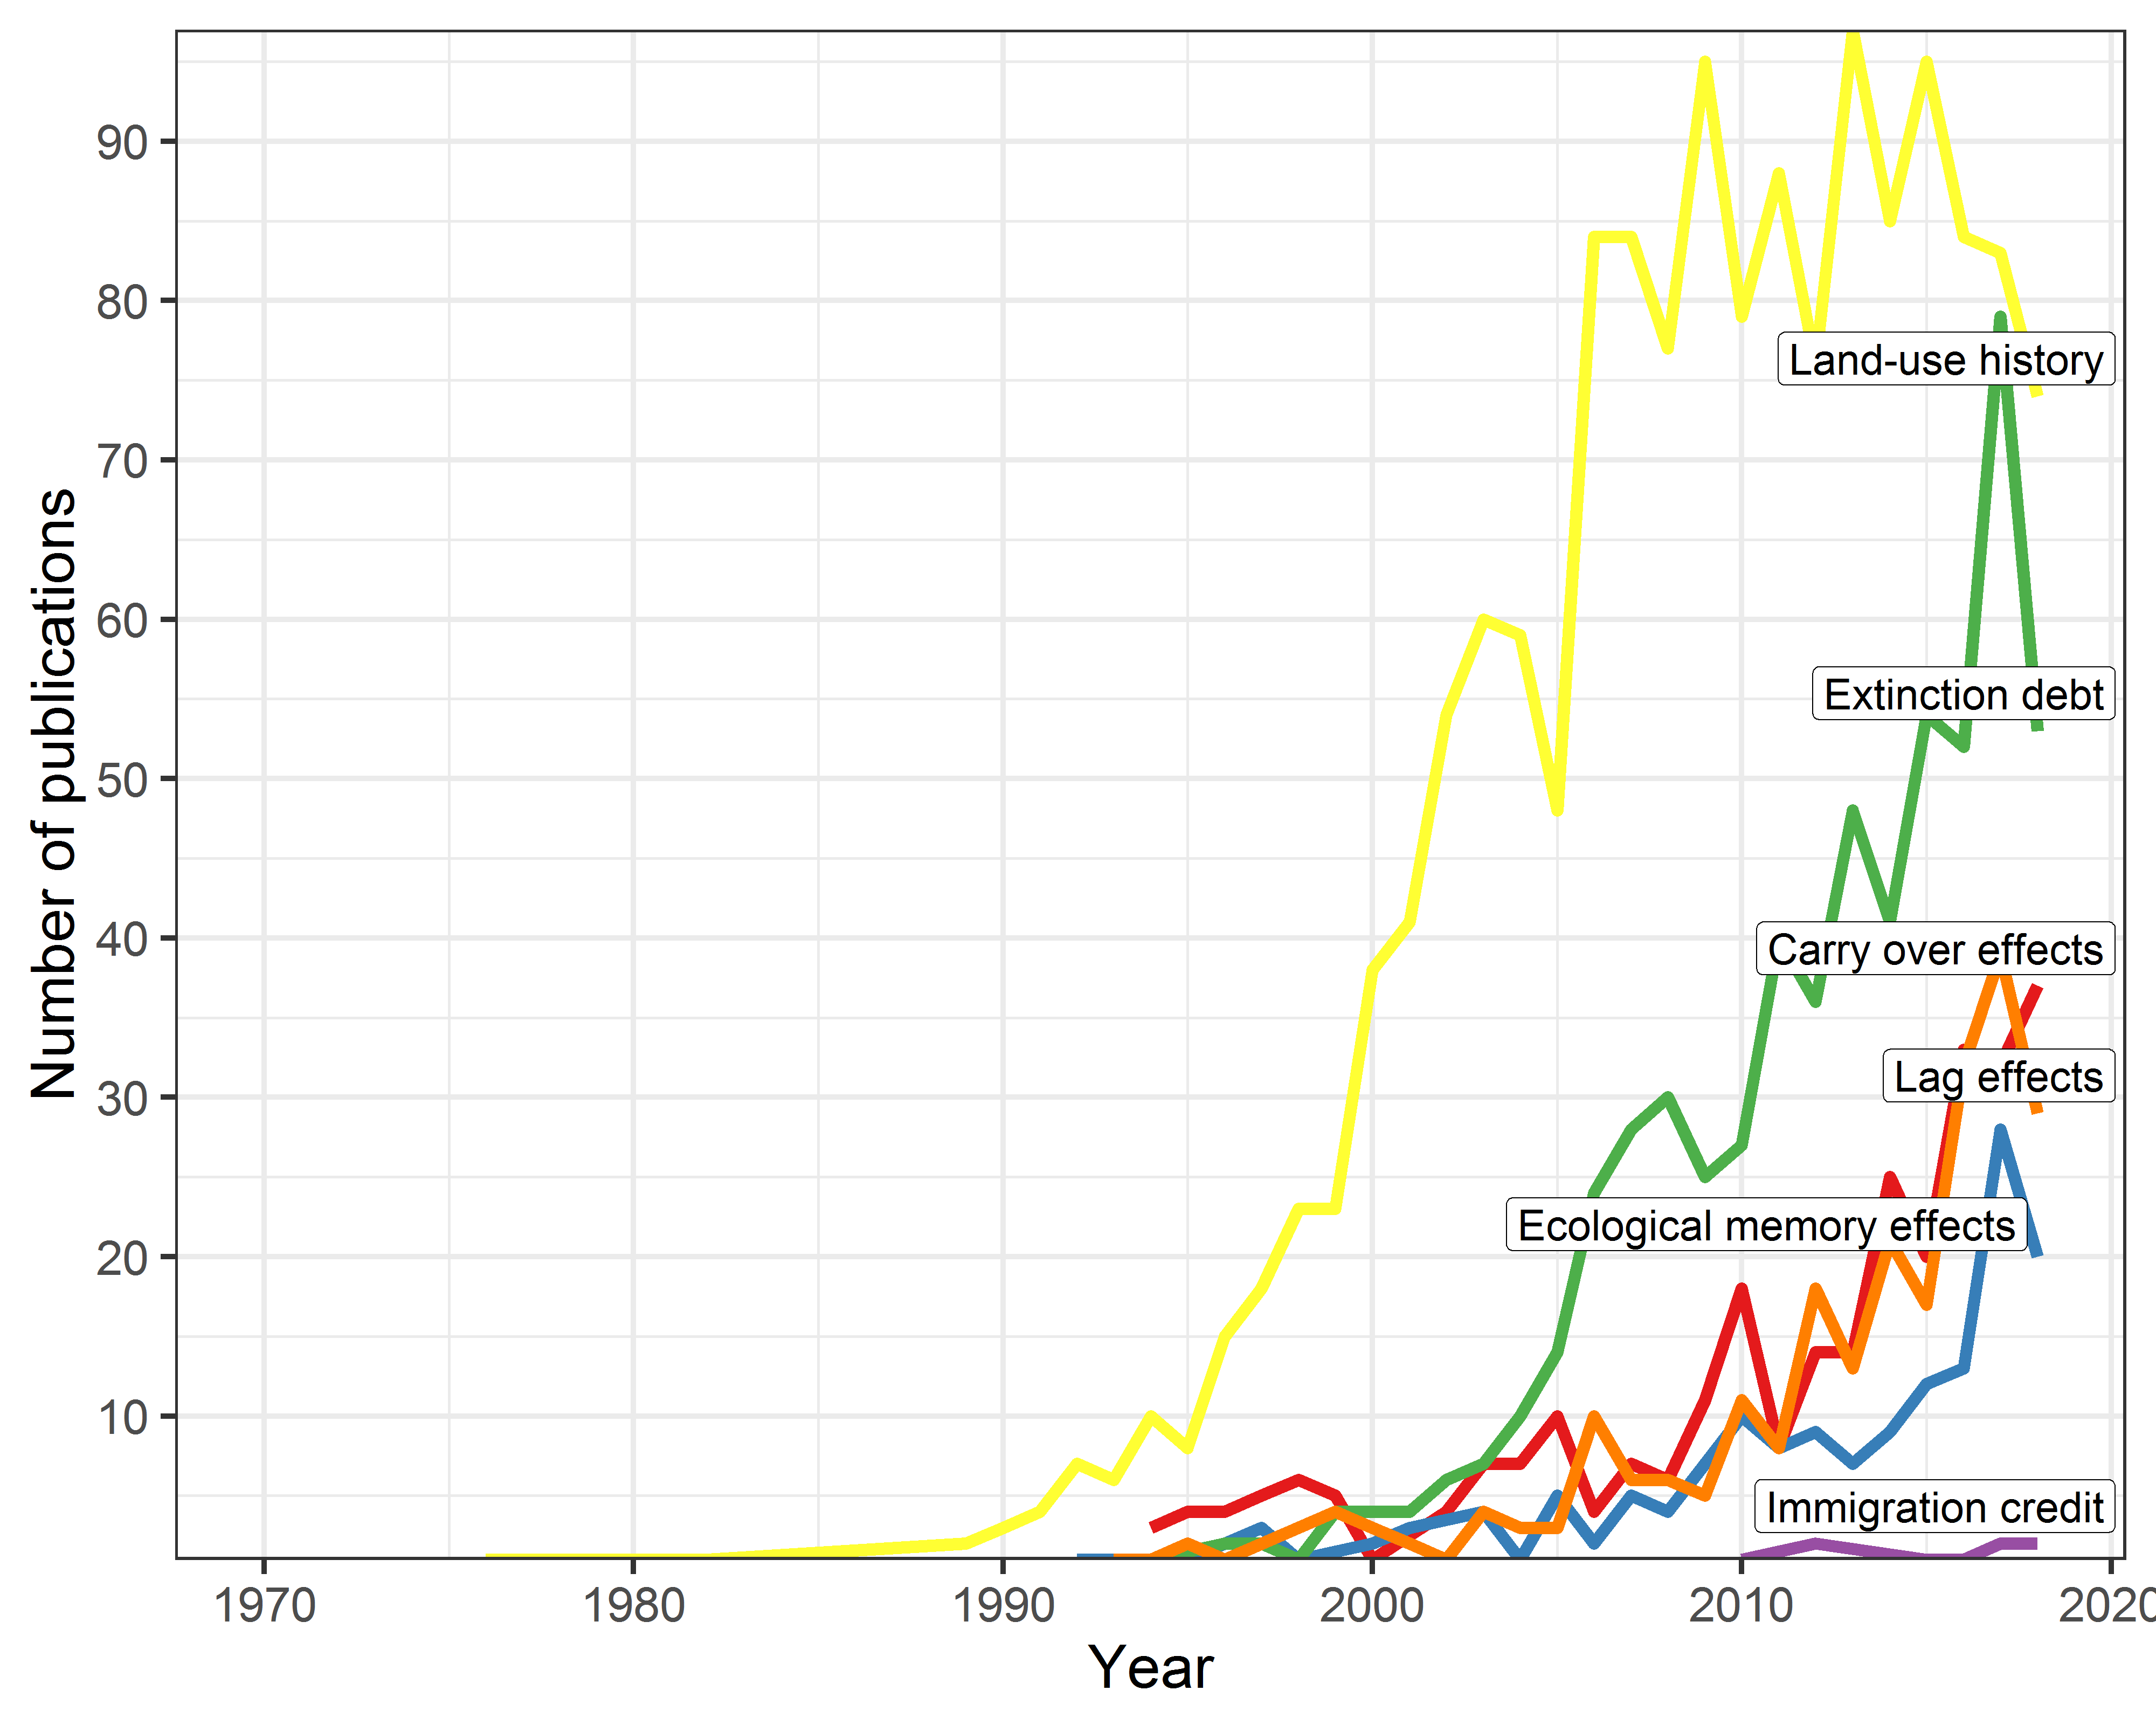
\includegraphics[width=1\textwidth]{chapter1/F04}
\caption{ Number of publications investigating terms and descriptions referring to biotic lag effects as queried from Web of Science\textsuperscript{TM} (WOS). A WOS search was conducted on the 5\textsuperscript{th} January 2019 limited to the Environmental sciences and ecological literature between 1900 and 2019 including as search topic “land-use histor*” (yellow), “extinction debt*” (green), “lag effect*” (orange), “carry*over effect*” (red), “ecological memory effect*” (blue) and “immigration credit*” (purple).  }
\label{F01_04}
\end{figure}
% -------------------------------------------- %

Several terms have been proposed to explain lasting impacts of past land change on local biodiversity (Table \ref{T01_01}). The term “extinction debt” describes the delayed extinction of species following a loss of habitat \citep{Balmford1996,Kuussaari2009,Wearn2012} and for many vertebrate species an extinction debt is usually “paid off” \textendash\ \eg the time until local population is fully extinct \textendash\ over a few years up to a century depending on the initial population size and species functional traits \citep{Halley2016}. Similarly, local biodiversity can also be influenced by an “immigration credit“, that is the delayed immigration of species from regional source populations after land change \citep{Jackson2010,Hylander2013}. Many species populations retain an “ecological memory” \citep{Peterson2002,Bengtsson2003,Ogle2015} of past land changes, reducing population growth and affecting species fitness and survival in subsequent years as “carry over” effect \citep{Harrison2011}. Collectively those terms can broadly be described as “biotic lag” effects (Table \ref{T01_01}), which are lasting or lagged effects of past changes in environmental factors that continue to influence present biodiversity. Knowledge about lasting impacts of land change can assist in planning management interventions \citep{Standish2014} and should be considered in broad-scale biodiversity models.  

Most existing regional and global assessments, models and scenarios of biodiversity \citep[\eg \ those included in the Intergovernmental Science-Policy Platform on Biodiversity and Ecosystem Services (IPBES) assessments, ][]{Alkemade2009,Pereira2010,Newbold2015} ignore lasting impacts of past land change. These assessments usually consider only concurrent differences in land-use/land-cover (Figure \ref{F01_03}) and may therefore partially misrepresent biodiversity change. Delayed impacts of past land change may accumulate together with other drivers \textendash\ such as climate change or species invasions \textendash\ of biodiversity change \citep{Essl2015,Essl2015a} potentially increasing the number of future species extinctions \citep{Dullinger2013}. To mediate the ongoing loss of biodiversity \citep{Mace2018}, robust estimates of the lasting impacts of land change on biodiversity need to be derived.

% ---------------- Table 1 ------------------- %
%\begin{landscape}
\begin{table}[ht]
\caption{Common terms and descriptions referring to lasting impacts of environmental changes on biodiversity}
\label{T01_01}

\newcolumntype{b}{X}
\newcolumntype{m}{>{\hsize=.6\hsize}X}
\newcolumntype{s}{>{\hsize=.4\hsize}X}

\begin{tabularx}{\textwidth}{ sbm }
\toprule
\textbf{Term} & \textbf{Description} & \textbf{Reference}   \\
\midrule

Land-use history  &  “Observed abiotic and biotic properties that are caused by past land use” & \citep{Foster2003,Perring2015} \\

Extinction debt & “The number of species committed to delayed extinction following a forcing event” &  \citep{Tilman1994,Kuussaari2009} \\

Immigration credit & “The number of species committed to delayed immigration following a forcing event” & \citep{Jackson2010} \\

Ecological memory & “The degree to which an ecological process is shaped by past modifications of the landscape, biotic and abiotic factors.” & \citep{Padisak1992,Peterson2002,Bengtsson2003,Ogle2015} \\

Carry-over effect & “Situation in which an individual’s previous history and experience explains their current performance in a given situation” & \citep{Harrison2011,OConnor2014} \\

Biotic lag &  Term summarizing the observed difference in biodiversity caused by lasting or lagged effects of past environmental changes  & \citep{DePalma2018} and this thesis   \\ \bottomrule

\end{tabularx}

\end{table}
% -------------------------------------------- %

\subsection{Linking satellite-based remotely-sensed land change with local biodiversity }
\label{C01_0103}

Remote sensing data can be useful for biodiversity models. Remotely-sensed land-surface conditions have been used to describe the biophysical state of species habitats \citep{Kerr2003}, identify critical life-history periods \citep{Pettorelli2005}, map species distributions \citep{He2015a} or as a proxy for predicting biodiversity patterns \citep{Rowhani2008,Rocchini2015,Hobi2017}. However, uncertainties remain in the usability of remote sensing data for different measures of biodiversity \citep{Oldeland2010}, for taxonomic groups \textendash\ where biodiversity measures are sometimes poorly correlated with photosynthetic activity \citep{Adler2011} or spectral dissimilarity \citep{Schmidtlein2017} \textendash\ or for many, previously unassessed geographic regions. Especially the temporal domain (Figure \ref{F01_02}\textbf{b}-\textbf{c}), including land change \textit{per se}, is often ignored \citep{Kennedy2014}. New frameworks are needed to establish links between remotely-sensed land change and local biodiversity.

Land change can be characterized by key attributes that may have varying impacts on local biodiversity (Figure \ref{F01_05}\textbf{a}). \cite{Watson2014} provided a conceptual framework that distinguishes between four attributes of land change: (\textbf{1}) The magnitude of land-change events, (\textbf{2}) the frequency of land-change events over time, (\textbf{3}) the time span since a land change occurred, and (\textbf{4}) the temporal sequence of land use and/or land cover categories (Figure \ref{F01_05}\textbf{a}). Ecological theory, experiments and simulations demonstrated that local biodiversity can be affected by these attributes (Figure \ref{F01_05}\textbf{b}). Land changes of larger magnitude are expected to affect biodiversity more \citep{Scheffer2001,Dornelas2010,Svensson2012,Ratajczak2018} and \textendash\ by removing poor dispersing \citep{Tilman1997} and specialist species \citep{Christensen2018} \textendash\ potentially reducing the stability of species assemblages \citep{Scheffer2001,Oliver2015,Hautier2015}. In many regions of the world, land changes vary in frequency \citep{Kleyer2007} impacting local biodiversity \citep{Valtonen2013,Lawson2015}, especially if those impacts accumulate in a short period of time \citep{Essl2015,Ratajczak2018}. Biodiversity measures can often recover to reference levels (\ie a temporal or spatial baseline) following land change, depending on the time passed \citep{Chazdon2003,Laurance2011,Martin2013}. Lastly, and commonly investigated, is the temporal sequence of land use and/or land cover types \citep{Harding1998,Chazdon2003,Foster2003}, where local biodiversity tends to be more altered at sites with past anthropogenic use. However, the impact of these four attributes of land change on local biodiversity has rarely been comparatively assessed globally and across taxonomic groups.

% ---------------- Figure 5 --------------------- %
\begin{figure}[htb]
\centering
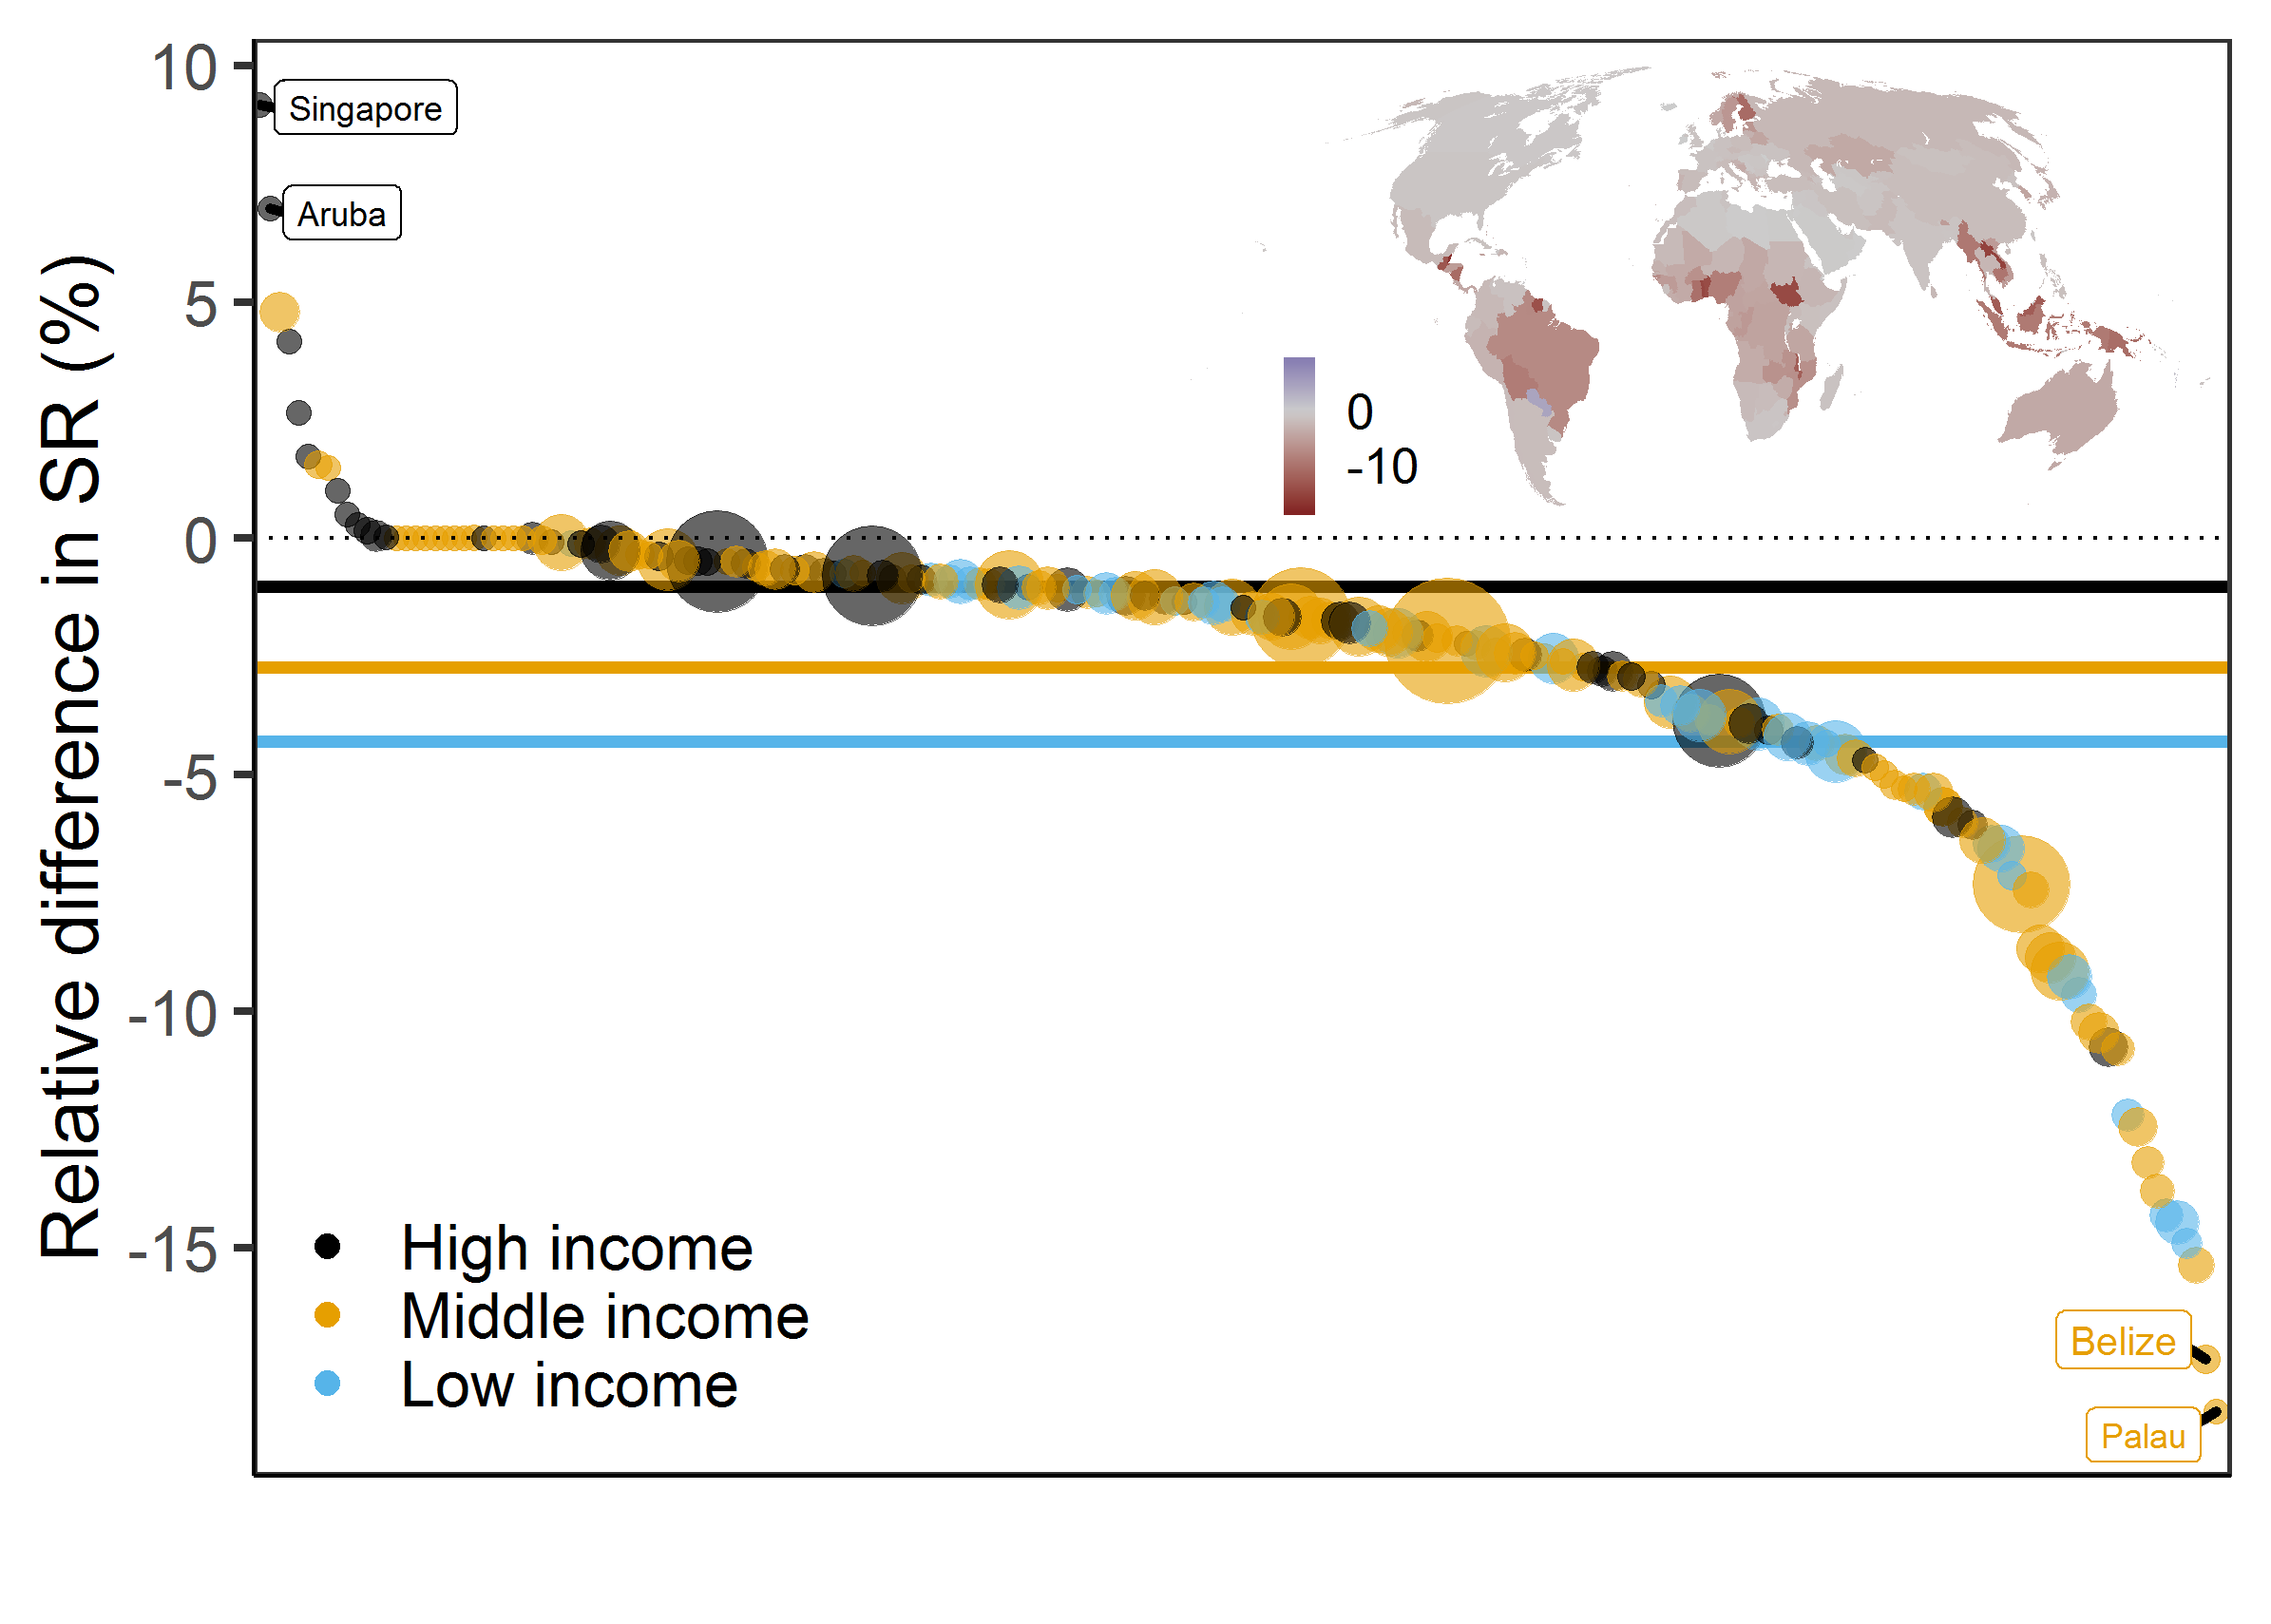
\includegraphics[width=1\textwidth]{chapter1/F05}
\caption{ (\textbf{a}) Conceptual framework \textendash\ inspired by \cite{Watson2014} \textendash\ how sites can differ by attributes of land change, namely (1) magnitude, (2) frequency, (3) time span and (4) sequence. Dashed lines indicate the start of biodiversity sampling with the y-axis representing an environmental predictor such as the Enhanced Vegetation Index (EVI). (\textbf{b}) Assumed response of biodiversity to varying land change attributes with x-axis indicating the strength of effect in units of each individual attribute.  }
\label{F01_05}
\end{figure}
% -------------------------------------------- %

\subsection{Thesis aims and structure}
\label{C01_0104}

The overall aim of my thesis is to investigate how local biodiversity is impacted by land changes globally and whether those impacts vary with attributes of land change  (Figure \ref{F01_05}). I do so by linking satellite-based remotely-sensed estimates of land change with measures of local biodiversity globally   (Figure \ref{F01_06}). The four main analytical chapters (Chapter \ref{C02}-\ref{C05}) of this thesis each address multiple of the four outlined attributes of land change (Figure \ref{F01_06}). They each serve as independent articles that have either been published, submitted or are in principle suitable for submission to an academic journal.

% ---------------- Figure 6 --------------------- %
\begin{figure}[htb]
\centering
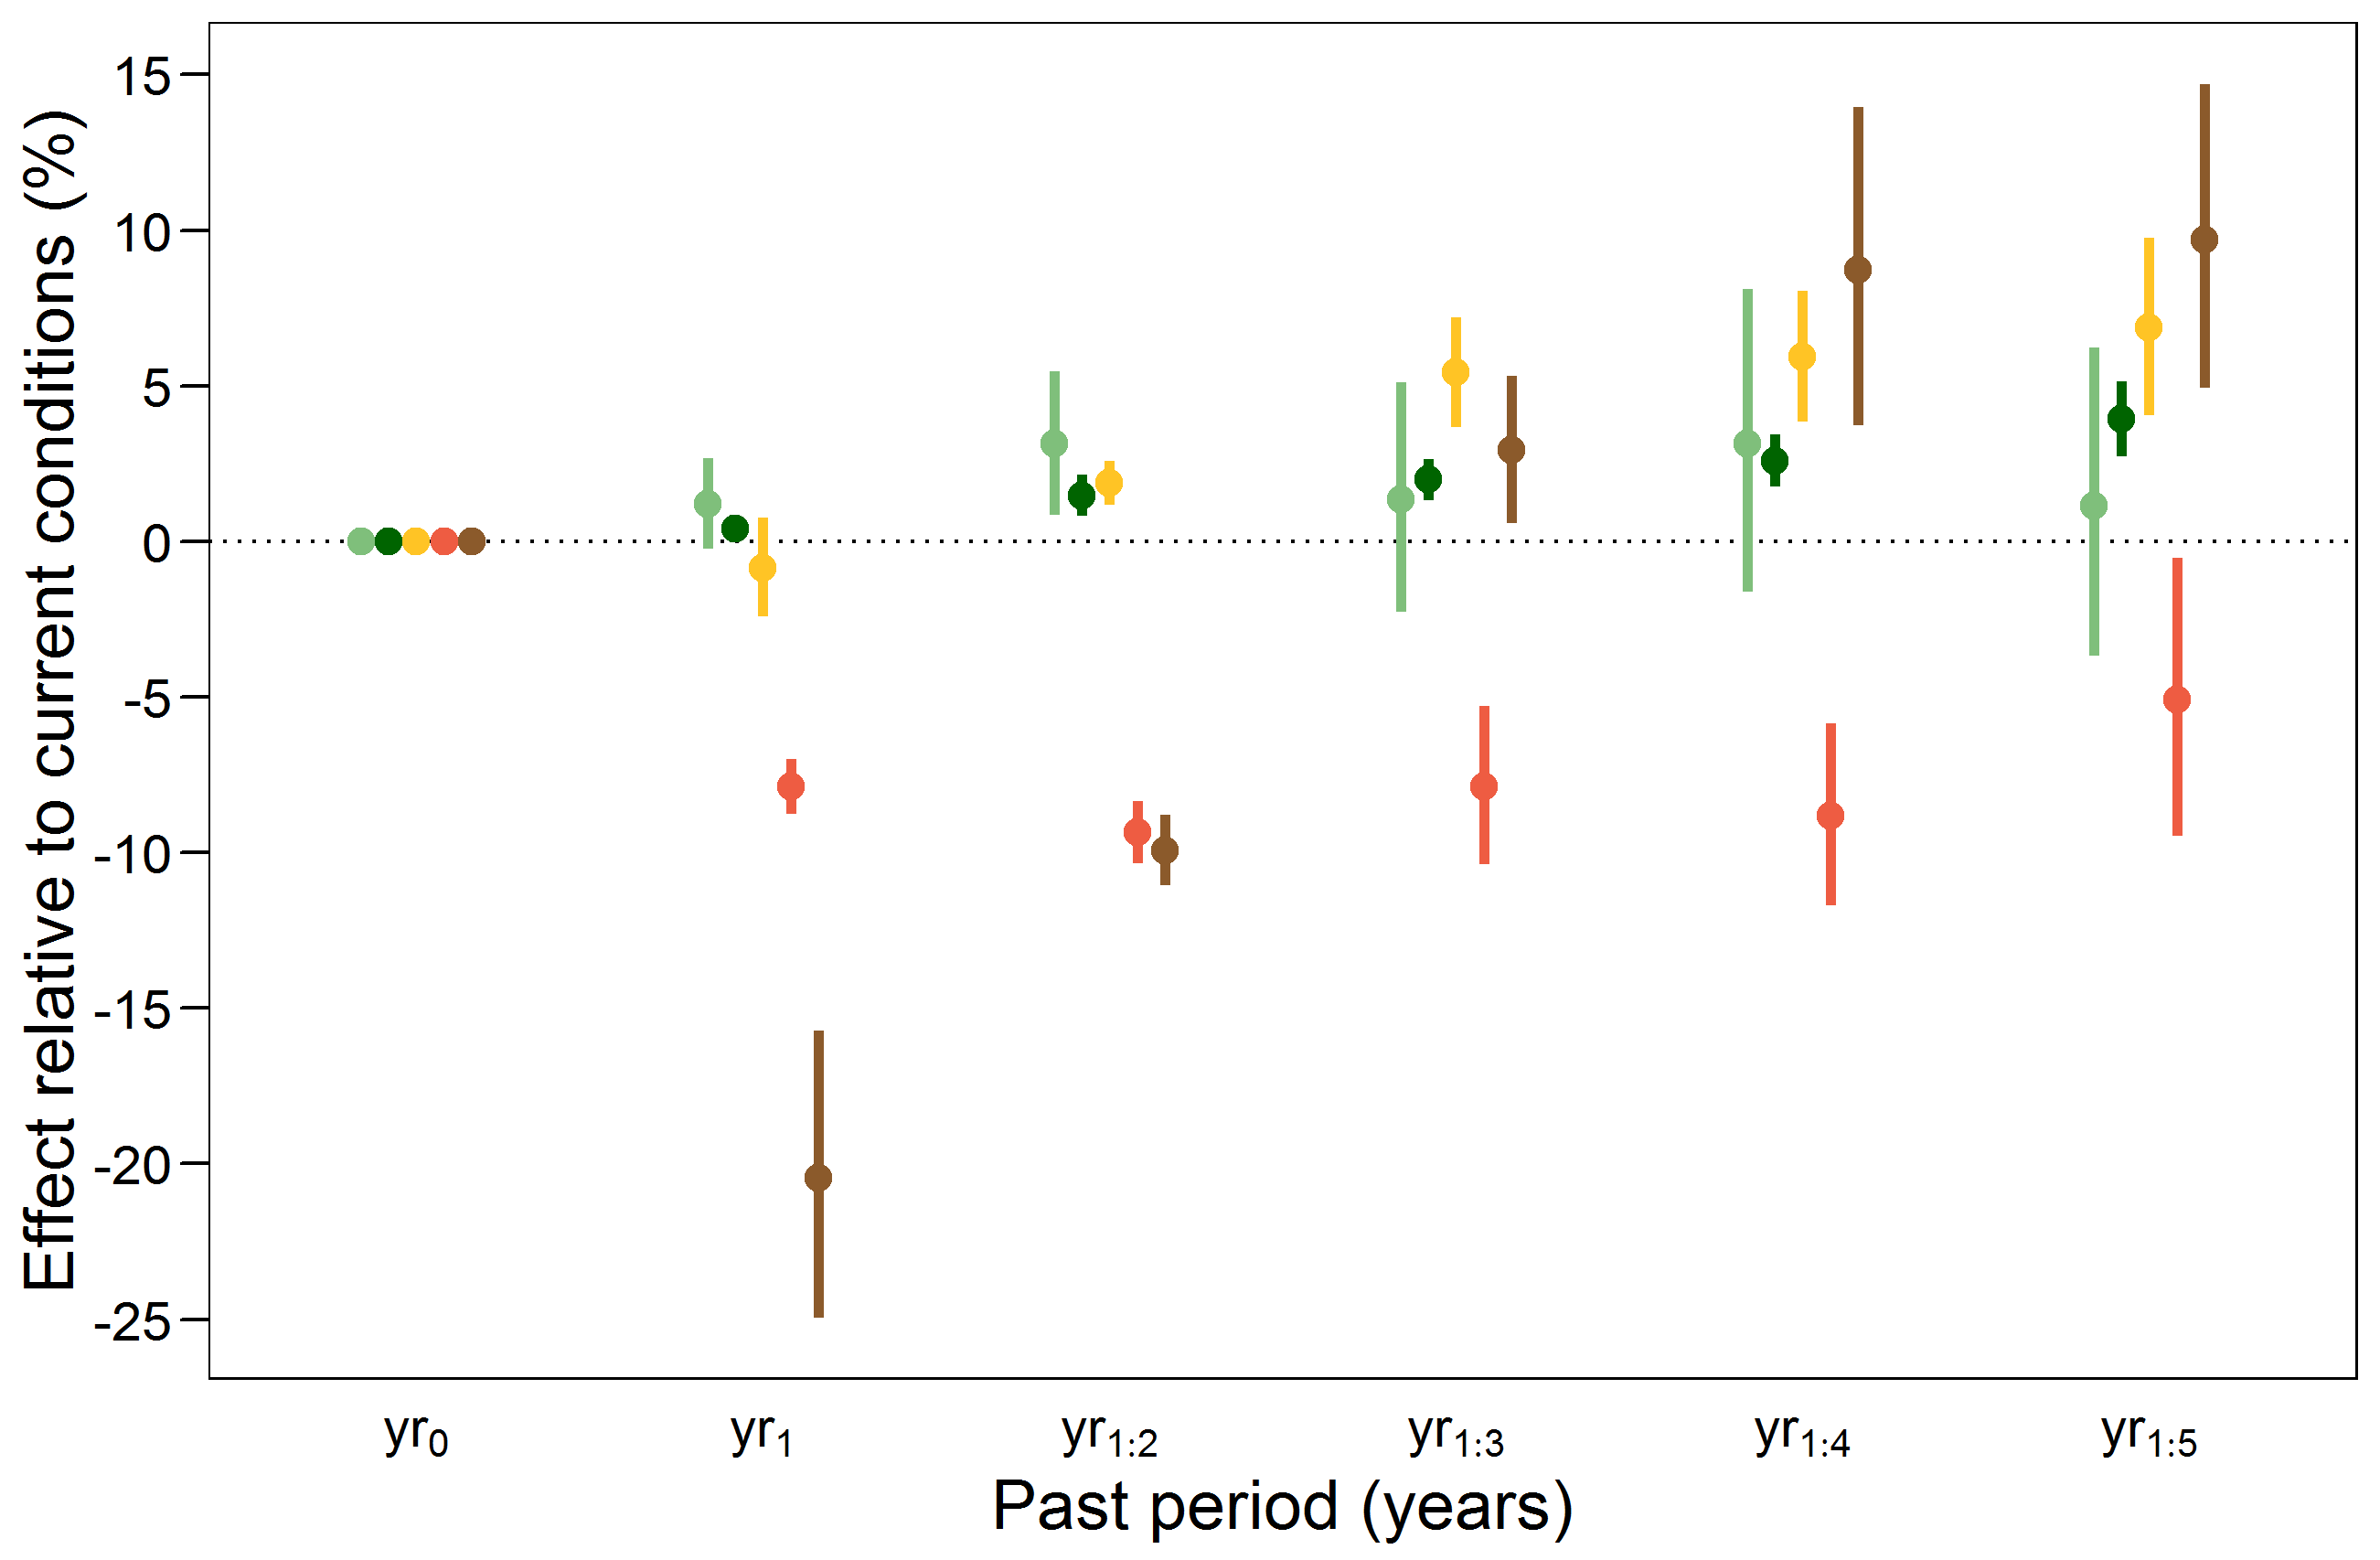
\includegraphics[width=1\textwidth]{chapter1/F06}
\caption{ Schematic outline of the four approaches (Chapter \ref{C02}-\ref{C05}) linking local biodiversity with remotely-sensed land change data, with lines and icons representing differences in intra-annual land dynamics (Chapter \ref{C02}), an abrupt land change of large magnitude (Chapter \ref{C03}), different land-cover sequences (Chapter \ref{C04}) and correlating temporal change in land and biodiversity observed at the same sites (Chapter \ref{C05}). Numbers in circles at the bottom left (1-4) indicate which attributes of land change from \cite{Watson2014} are considered in each approach (see Figure \ref{F01_05}\textbf{a}), while logos indicate the biodiversity data used (PREDICTS or United States BBS data). }
\label{F01_06}
\end{figure}
% -------------------------------------------- %

Chapter two assesses whether considering past land-surface conditions in the six years before biodiversity sampling can assist in explaining differences in local biodiversity. I developed an analytical framework that captures all differences between time series of remotely-sensed land-surface conditions \textendash\ such as land changes with varying magnitude or inter-annual frequency \textendash\ in a single metric, which was then linked with differences in species assemblage composition across taxonomic and functional groups globally. 

The third chapter focusses on how abrupt land changes \textendash\ characterized by shifts in magnitude or trend and varying time passed \textendash\ continue to influence local biodiversity. I assembled time series of Landsat imagery globally (Figure \ref{F01_01}\textbf{a}) and subjected them to a change-detection algorithm to detect abrupt land changes. A hierarchical analysis was conducted to assess if and how strongly local biodiversity differs between sites with and without a land change in the past. The assumption is that local biodiversity is more affected by abrupt land changes of greater magnitude that occurred more recently.

In chapter four I investigated how local biodiversity differs between sites with varying land-cover sequences of land cover change as derived from a global, temporally consistent land-cover product for the years 1992 to 2015. The assumption is that local biodiversity is higher at sites with a past land-cover change compared to those without, if the preceding land cover was less anthropogenically modified. In addition, this chapter investigates how past land-cover sequences can influence global and national biodiversity projections and argues for including estimates of past land change in biodiversity projections.

In contrast to previous chapters, in the fifth chapter I investigate if local biodiversity change can be linked to landscape-wide land changes. Estimates of bird diversity change from repeated breeding bird surveys (BBS data, Figure \ref{F01_01}) were correlated with estimates of preceding and concurrent land change at the landscape scale quantified from time series of Landsat imagery. I furthermore investigate whether the explanatory power of landscape-wide land changes on bird diversity change varies in space, time and across functional groups of bird species. The assumption is that bird diversity declines more in landscapes with a greater proportion of land changes.

The thesis concludes with the sixth chapter, which provides a synthesis of the presented work, discusses all findings in relation to previous studies, and mentions shortcomings and promising directions for future research.

\clearpage
%\bibliography{content/01Chapter}

%\appendix
%\begingroup
%  Blank

%\endgroup
